\chapter{Povezivanje razvojnog sustava i oblaka}

Oblak koju pruža platforma AWS i razvojni sustav ESP32-C3 dva su odvojena sustava koja moraju međusobno komunicirati i razmjenjivati podatke. Za ostvarenje njihove veze razvijena su dva programska rješenja:
\begin{enumerate}
	\item programska potpora za mikrokontroler, koja će omogućiti dinamičko povezivanje na Wi-Fi, spajanje na platformu AWS te slanje podataka u oblak,
	\item programska potpora za platformu AWS, koja će ostvariti umrežavanje uređaja u sustav, ažuriranje softvera na uređaju, pohranu primljenih podataka s uređaja te prikaz tih podataka u web aplikaciji. 
\end{enumerate} 

\section{Programska potpora za mikrokontroler}

Programska potpora za uređaj ESP32-C3 sastoji se od nekoliko komponenti:
\begin{itemize}
	\item dinamičko povezivanje na bežičnu mrežu,
	\item spajanje na platformu AWS,
	\item učitavanje novog softvera, 
	\item očitavanje senzorskih mjerenja, 
	\item slanje podataka u oblak protokolom MQTT.
\end{itemize}

Neke od navedenih komponenti izvršavaju se slijedno, dok se druge izvršavaju paralelno. Spajanje na Wi-Fi i povezivanje s platformom AWS ključni su koraci koji prethode bilo kakvom pokušaju slanja podataka u oblak. Isto tako, praćenje ažuriranja softvera i očitavanje mjerenja izvršavaju se paralelno u posebnim procesima budući da nisu sekvencijalni niti međusobno isključivi zadaci. U nastavku je pobliže opisan svaki navedeni segment programske potpore. 

\subsection{Dinamičko povezivanje mikrokontrolera na Wi-Fi}

Radni okvir ESP-IDF nudi dinamičko spajanje na Wi-Fi mrežu pomoću zasebne komponente. Ovaj se postupak naziva provizioniranje \engl{provisioning}. Ova komponenta pruža aplikacijska programska sučelja \engl{Application Programming Interface - API} koja kontroliraju pružanje usluge za primanje i konfiguriranje Wi-Fi vjerodajnica putem sigurnih komunikacijskih protokola. Sigurnosni protokoli definirani su u komponenti protokolne komunikacije \engl{protocomm} koja upravlja sigurnim sjednicama \engl{sessions} i pruža radni okvir za višestruki prijenos podataka. Također je moguće direktno koristiti sloj \textit{protocomm} radi implementacije specifične za aplikaciju. \cite{unified_provisioning}

Sloj \textit{protocomm} interno koristi mehanizam protokolnih međuspremnika \engl{protocol buffers - protobuf} za sigurno uspostavljanje sjednice. Protokolni međuspremnici namijenjeni su za serijalizaciju strukturiranih podataka neovisno o programskom jeziku i platformi. Koristan je pri izradi programa i sustava koji međusobno komuniciraju putem mreže zbog kompaktnosti i niske latencije. \cite{what_is_protobuf}

Sloj \textit{protocomm} pruža radni okvir za različite načine komunikacije:
\begin{enumerate}
	\item protokol BLE,
	\item Wi-Fi (SoftAP u kombinaciji s HTTP serverom).
\end{enumerate}

Pružajući korisnicima okvir za ostvarivanje usluge dinamičkog povezivanja u mrežu, neovisno o načinu komunikacije, ovakva vrsta podrške naziva se unificirano provizioniranje \engl{unified provisioning}. Ovakav način prijave uređaja na mrežu zahtijeva interakciju korisnika putem vanjskog uređaja za slanje vjerodajnica na mikrokontroler. Tvrtka \textit{Espressif} pruža jednostavna mobilna rješenja koja se mogu koristiti gotova ili pak uklopiti u vlastitu mobilnu aplikaciju. Na slici \ref{fig:unified_provisioning} prikazana je arhitektura usluge.

\begin{figure}[ht]
	\centering
	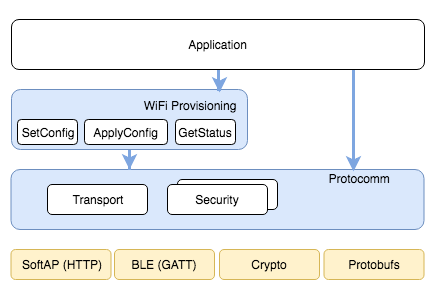
\includegraphics[scale=0.8]{imgs/unified_provisioning}
	\caption{Arhitektura unificiranog provizioniranja \cite{unified_provisioning}}
	\label{fig:unified_provisioning}
\end{figure}

Kao što je ranije opisano, arhitektura je bazirana na sloju \textit{protocomm} koji je odgovoran za prijenos podataka i sigurnost. Služi za jednostavne povratne pozive aplikaciji \engl{callbacks} i dobivanje Wi-Fi statusa. Sama aplikacija ima kontrolu nad implementacijom povratnih poziva. 

Aplikacija stvara instancu \textit{protocomm} koja se preslikava na određeni prijenosni protokol i sigurnosnu shemu. Svaki prijenos podataka u sloju \textit{protocomm} ima koncept krajnje točke \engl{endpoint} koji odgovara logičkom komunikacijskom kanalu za određenu vrstu informacija. Primjerice, sigurnosno rukovanje \engl{handshake} odvija se na različitoj krajnjoj točki u odnosu na točku za Wi-Fi konfiguraciju. Svaka se krajnja točka identificira nizom znakova i mijenja se ovisno o internom prikazu krajnje točke. U slučaju prijenosa pomoću Wi-Fi veze odnosno SoftAP funkcionalnosti, krajnja točka prikazuje se kao URI, dok u slučaju prijenosa podataka putem protokola BLE odgovara GATT karakteristici sa specifičnim UUID-om. 

Oglašavanje i otkrivanje uređaja prepušteno je aplikaciji i ovisno o odabranom protokolu, vanjske aplikacije mogu odabrati odgovarajuću metodu za oglašavanje i otkrivanje. Za Wi-Fi prijenos obično se koristi ime mreže pristupne točke. Za prijenos putem protokola BLE može se koristiti ime samog uređaja. 

Kao što je opisano, podržano je korištenje protokola BLE kao i Wi-Fi usluge za prijenos vjerodajnica. Pri odabiru prijenosnog kanala za spajanje uređaja u mrežu, potrebno je razmotriti nekoliko točaka. Za početak, prijenos temeljen na protokolu BLE prednost održavanja netaknutog komunikacijskog kanala između uređaja i klijenta tijekom prijenosa podataka, što osigurava pouzdanu povratnu informaciju. S druge strane, prijenos putem Bluetootha troši oko 110 KB memorije tijekom rada, što je na uređajima niskih resursa velika potrošnja. Korisno je što se korištena memorija može vratiti na hrpu \engl{heap} po završetku umrežavanja uređaja ukoliko se BLE funkcionalnosti više ne koriste. Prijenos temeljen na Wi-Fi mreži, odnosno SoftAP funkcionalnosti, vrlo je interoperabilan i ne troši dodatnu memoriju. Međutim, mikrokontroler koristi isti radio za emitiranje pristupne točke i za spajanje na željenu mrežu. Budući da se te akcije mogu odvijati na različitim kanalima, postoji mogućnost da se ažuriranja statusa veze ne dostave na mobilni uređaj. Također, mobilni se uređaj mora odspojiti s izvorne Wi-Fi mreže radi privremenog spajanja na pristupnu točku mikrokontrolera. Uređaj će se spojiti na izvornu mrežu tak kada mikrokontroler ugasi pristupnu točku. 

Za razvoj predloženog rješenja korišteno je slanje vjerodajnica pomoću Wi-Fi mreže, odnosno privremene pristupne točke. Kao što je ranije opisano, protokol BLE troši značajnu količinu \textit{heap} memorije, a razvojni sustav ESP32-C3 nema dovoljno radne memorije koja bi pokrila prijavu u mrežu uz ostale radne procese. Mikrokontroler najprije stvori privremenu pristupnu točku na koju se mobilni uređaj spaja pomoću mobilne aplikacije. Zatim, nakon skeniranja dostupnih Wi-Fi mreža u blizini, u mobilnoj aplikaciji odabire se željena mreža i unese lozinka. Vjerodajnice se zatim pošalju putem Wi-Fi mreže, i mobilni uređaj može se odspojiti s privremene pristupne točke. Vjerodajnice se pohrane u memoriju tipa NVS \engl{non-volatile storage} koja ne zahtijeva konstantno napajanje kako bi se zadržala na uređaju. Ovime je omogućeno povezivanje uređaja u sustav čak i kada dođe do prekida napajanja. \cite{what_is_nvs} Memorija tipa NVS može se jedino programski obrisati, te bi u idealnom izvedbenom rješenju postojao vanjski gumb spojen na mikrokontroler koji bi pokretao brisanje te memorije i tako omogućio ponovno spajanje na željenu mrežu. Sljedeći programski isječak prikazuje inicijalizaciju memorije NVS, mrežnog sučelja te stvaranje pristupne točke.

\begin{lstlisting}[caption={Stvaranje pristupne točke}, language=c]
	/* Init NVS partition */
	esp_err_t ret = nvs_flash_init();
	/* Init TCP/IP */
	ESP_ERROR_CHECK(esp_netif_init());
	/* Init the event loop */
	ESP_ERROR_CHECK(esp_event_loop_create_default());
	wifi_event_group = xEventGroupCreate();
	/* Init Wi-Fi including netif with default config */
	esp_netif_create_default_wifi_sta();
	esp_netif_create_default_wifi_ap();
	wifi_prov_mgr_config_t config = {
		.scheme = wifi_prov_scheme_softap,
		.scheme_event_handler = WIFI_PROV_EVENT_HANDLER_NONE
	};
    /* Init provisioning manager with above config */
	ESP_ERROR_CHECK(wifi_prov_mgr_init(config));
	ESP_ERROR_CHECK(wifi_prov_mgr_start_provisioning(security, (const void *) sec_params, service_name, service_key));
	wifi_prov_print_qr(service_name, username, pop, PROV_TRANSPORT_SOFTAP, disp);
\end{lstlisting}

\subsubsection{LCD zaslon}

Za povezivanje mobilnog uređaja na privremenu pristupnu točku koju emitira razvojni sustav, potrebno je skenirati QR kod koji mikrokontroler generira. Budući da ESP32-C3 nema vlastito sučelje, na sustav je spojen zaslon OLED SSD1306 veličine 128×64 piksela. Uređaj sa zaslonom komunicira putem I2C sučelja, a za prikaz sadržaja na zaslonu korištena je biblioteka LVGL \engl{Light and Versatile Graphics Library}. To je grafička biblioteka otvorenog koda namijenjena izradi GUI aplikacija za ugradbene sustave. Pruža radni okvir s mnogim značajkama, temama i paletama boja. Isto tako, biblioteka troši vrlo malo resursa, što je čini pogodnom za uređaje poput razvojnog sustava ESP32-C3. \cite{lvgl} Generiranje QR koda obavlja se pomoću biblioteke \textit{QR-Code-Generator} koja je prilagođena ESP32 uređajima. 

\begin{lstlisting}[caption={Generiranje QR koda iz pristupne točke}, language=c]
static void wifi_prov_print_qr(const char *name, const char *usrname, const char *pop, const char *transport, lv_disp_t *disp) {
	char payload[150] = {0};
    snprintf(payload, sizeof(payload), 	
    	"{\"ver\":\"%s\",\"name\":\"%s\",\"username\":\"%s\",\"pop\":\"%s\",\"transport\":\"%s\"}",
    	 PROV_QR_VERSION, name, usrname, pop, transport);
    esp_qrcode_config_t cfg = {
		.display_func = generate_qr_code_lcd, 
		.max_qrcode_version = 10, 
		.qrcode_ecc_level = ESP_QRCODE_ECC_LOW
	};
	esp_qrcode_generate(&cfg, payload);
}
\end{lstlisting}

Prethodna funkcija povezuje pristupnu točku s QR kodom. Podaci o samoj pristupnoj točki učitaju se u privremenu varijablu, čiji se sadržaj prosljeđuje biblioteci za generiranje QR koda. Dobiveni se podaci zatim prosljeđuju funkciji za prikaz koda na zaslonu. QR kod prikazuje se na zaslonu piksel po piksel, skalirajući veličinu QR koda na temelju širine i duljine samog zaslona. 

\begin{lstlisting}[caption={Funkcija za prikaz QR koda na zaslonu}, language=c]
void generate_qr_code_lcd(esp_qrcode_handle_t qrcode)
{
	ESP_LOGI(TAG, "%s", "Started generate_qr_code_lcd...");
	
	int size = qrcodegen_getSize(qrcode);
	
	// Calculate the scale factor
	int scale = (int)fmin(EXAMPLE_LCD_H_RES / size, EXAMPLE_LCD_V_RES / size);
	
	// Calculate horizontal shift
	int shift_x = (EXAMPLE_LCD_H_RES - size * scale)/2;
	
	// Calculate vertical shift
	int shift_y = (EXAMPLE_LCD_V_RES - size * scale)/2;
	
	if (lvgl_port_lock(0)) {
		lv_obj_t *screen = lv_scr_act();
		lv_obj_clean(screen); // Clear the screen to ensure it's dark
		
		// Create a canvas object
		lv_obj_t *canvas = lv_canvas_create(screen);
		static lv_color_t cbuf[LV_CANVAS_BUF_SIZE_TRUE_COLOR(EXAMPLE_LCD_H_RES, EXAMPLE_LCD_V_RES)];
		lv_canvas_set_buffer(canvas, cbuf, EXAMPLE_LCD_H_RES, EXAMPLE_LCD_V_RES, LV_IMG_CF_TRUE_COLOR);
		lv_canvas_fill_bg(canvas, lv_color_white(), LV_OPA_COVER);
		
		// Draw the QR code on the canvas
		for (uint8_t y = 0; y < size; y++) {
			for (uint8_t x = 0; x < size; x++) {
				if (qrcodegen_getModule(qrcode, x, y)) {
					for (int dy = 0; dy < scale; dy++) {
						for (int dx = 0; dx < scale; dx++) {
							lv_canvas_set_px(canvas, shift_x + x * scale + dx, shift_y + y * scale + dy, lv_color_black());
						}
					}
				}
			}
		}
		
		// Release the mutex
		lvgl_port_unlock();
	}
}
\end{lstlisting}

Na slici \ref{fig:esp32_lcd} prikazan je razvojni sustav ESP32-C3 sa spojenim LCD zaslonom na kojem je prikazan generirani QR kod.

\begin{figure}[ht]
	\centering
	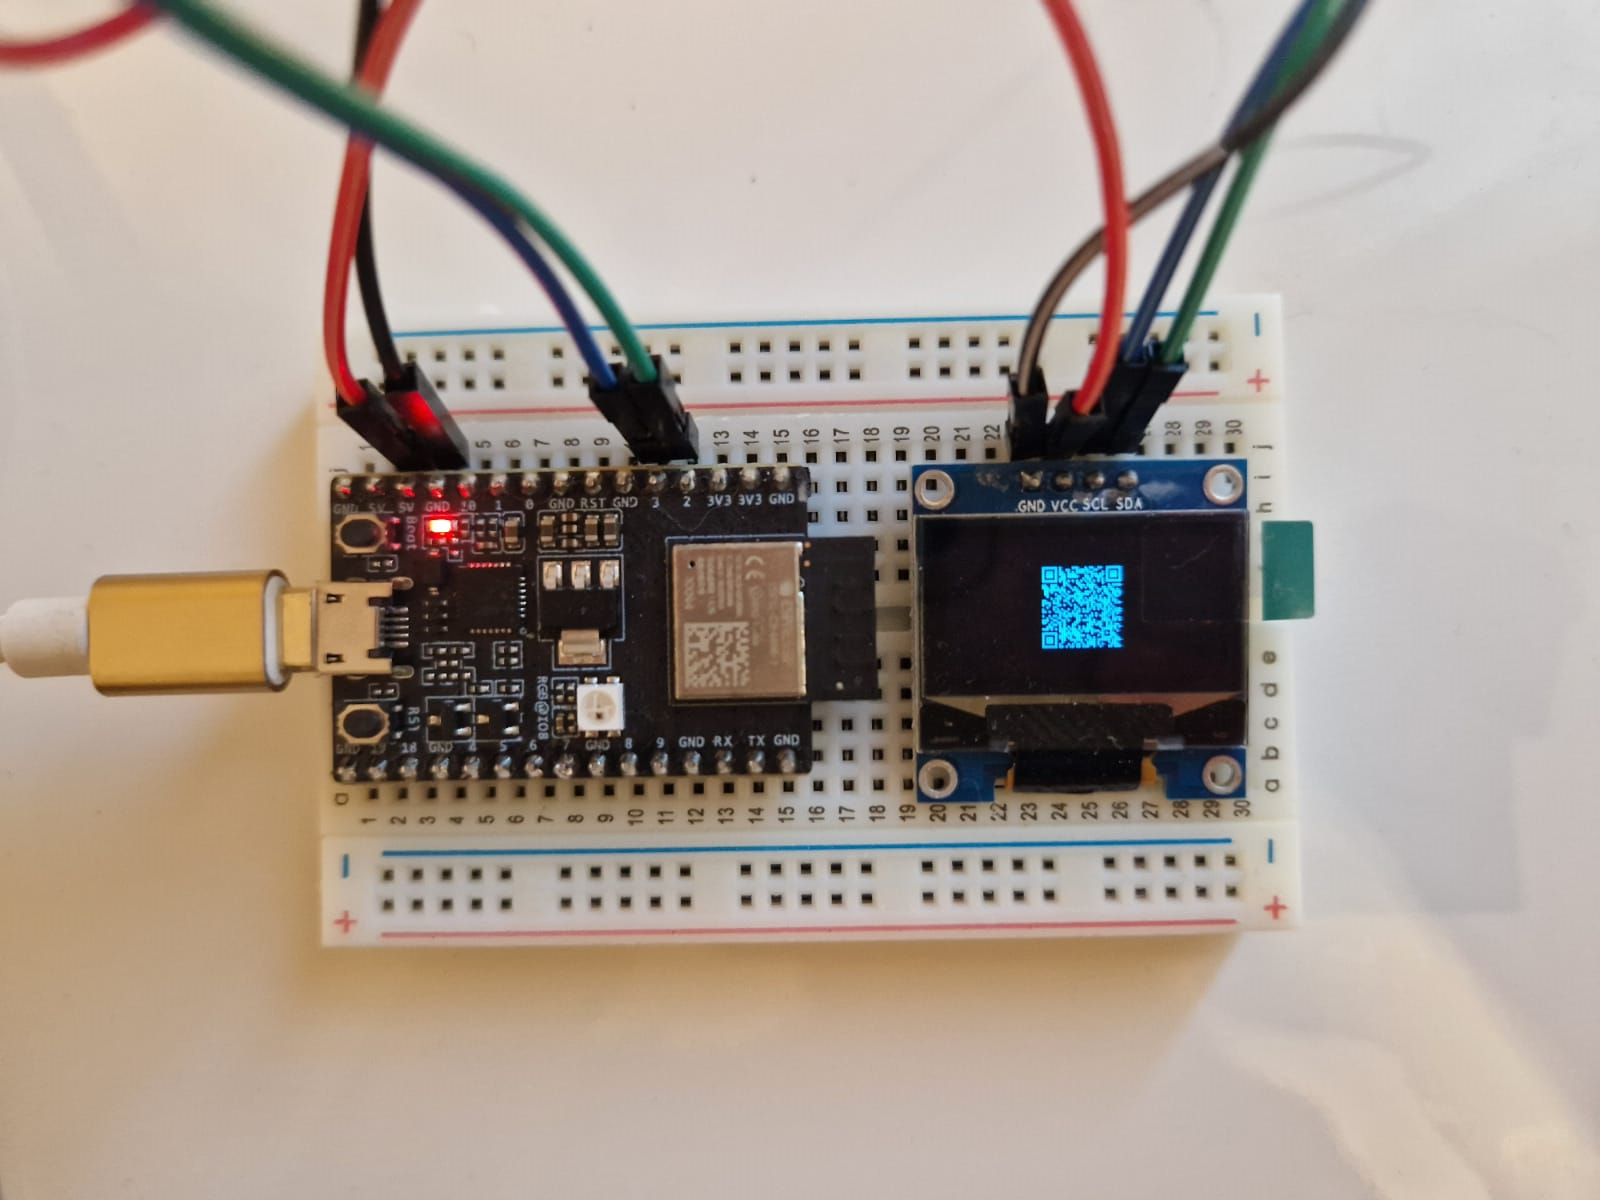
\includegraphics[scale=0.3]{imgs/esp32_lcd}
	\caption{Razvojni sustav spojen s LCD zaslonom}
	\label{fig:esp32_lcd}
\end{figure}

\subsection{Registracija u sustav AWS}

\section{Programska potpora za oblak}

Ovdje će trebati dosta toga navesti, odnosno koji su koraci napravljeni u samom AWS sustavu da bi se mikrokontroler uspješno spojio s AWS-om. Vjerojatno opisati korake kreiranja računa, stvaranja certifikata koji će se zatim posijati u uređaj itd. 

\subsection{Povezivanje s mikrokontrolerom}

Ovdje će trebati opisati cijeli flow kojim se mikrokontroler spaja na AWS.